\chapter{Laboratory Study Materials}

%%%%%%%%%%%%%%%%%%%%%%%%%%%%%%%%%%%%%%%%%%%%%%%%%%%%%%%%%%%%%%%%%%%%%%

\section{Briefing and Setup Instructions}
\label{sec:Briefing-and-Setup}

\subsection{Briefing}
\label{subsec:Briefing}

Apache Kafka is an event streaming platform used to collect, process, and store streaming event data that has no discrete beginning or end, \eg real-time stock trades and social media feeds. 
As part of Kafka’s contribution guidelines, a commit’s title/subject is usually of the form ``KAFKA-XXXX: Title,'' where ``KAFKA-XXXX'' is the relevant Jira issue ID and ``Title'' may be the Jira’s title or a more specific title describing the pull request itself. 
For trivial cases where a Jira issue is not required, ``MINOR:'' or ``HOTFIX:'' is used as the commit’s title prefix.

In this study, you will be exploring two Java classes and their commit histories from the Kafka project and answering a series of questions in a semi-structured interview format. The process of finding the answers to these questions can involve reading the commit messages for commits and visiting the relevant Jira issue on Apache’s Jira instance:
\url{https://issues.apache.org/jira/browse/KAFKA-XXXX}.

You may also see the acronym ``KIP'' referenced in some commits or Jira issues in Kafka. You may use and reference KIPs in your exploration and answers. These are Kafka Improvement Proposals (\entity{KIP}s) and can be found at: 
\url{https://cwiki.apache.org/confluence/display/kafka/kafka+improvement+proposals}.

\subsection{Setup Instructions}
\label{sec:Setup-Instructions}

\begin{enumerate}
    \item Install IntelliJ IDEA, either Community (free) or Ultimate edition (if you already have a license). See: \url{https://www.jetbrains.com/idea}. If you already have IntelliJ installed, please confirm the version number. The version must be 2022.1 or greater, which you can verify by navigating to the top bar  ``Help'' → ``About'' (Windows) or top bar → ``IntelliJ IDEA'' → ``About IntelliJ IDEA'' (Mac).
    \item Clone the Apache Kafka repository (roughly 200 MB on disk) or you can request the co-investigator to provide a ZIP of the repository: 
    
    \begin{center}
        \code{git clone --single-branch --branch trunk https://github.com/apache/kafka.git}
    \end{center}

    \item Open the Kafka project in IntelliJ: ``File'' → ``Open''
    \item To install the plugin, download \code{Intelligent.History-1.0.0.zip} at: \url{https://github.com/Alison-Li/intelligent-history/releases/tag/v1.0.0-eval}. Go to “Settings/Preferences” → ``Plugins'' → Gear Icon → ``Install Plugin from Disk\dots''
    \item For the task involving the plugin: Go to ``Settings/Preferences'' → ``Tools'' → ``Intelligent History'' to configure the Jira settings. Alternatively, go to “Settings/Preferences’ → type ``Intelligent History'' in the search field to look for the plugin settings. The co-investigator will provide you with the information needed to fill in the fields.
\end{enumerate}

%%%%%%%%%%%%%%%%%%%%%%%%%%%%%%%%%%%%%%%%%%%%%%%%%%%%%%%%%%%%%%%%%%%%%%

\pagebreak

\section{Session Summaries}
\label{sec:Summaries}

\begin{figure}[H]
    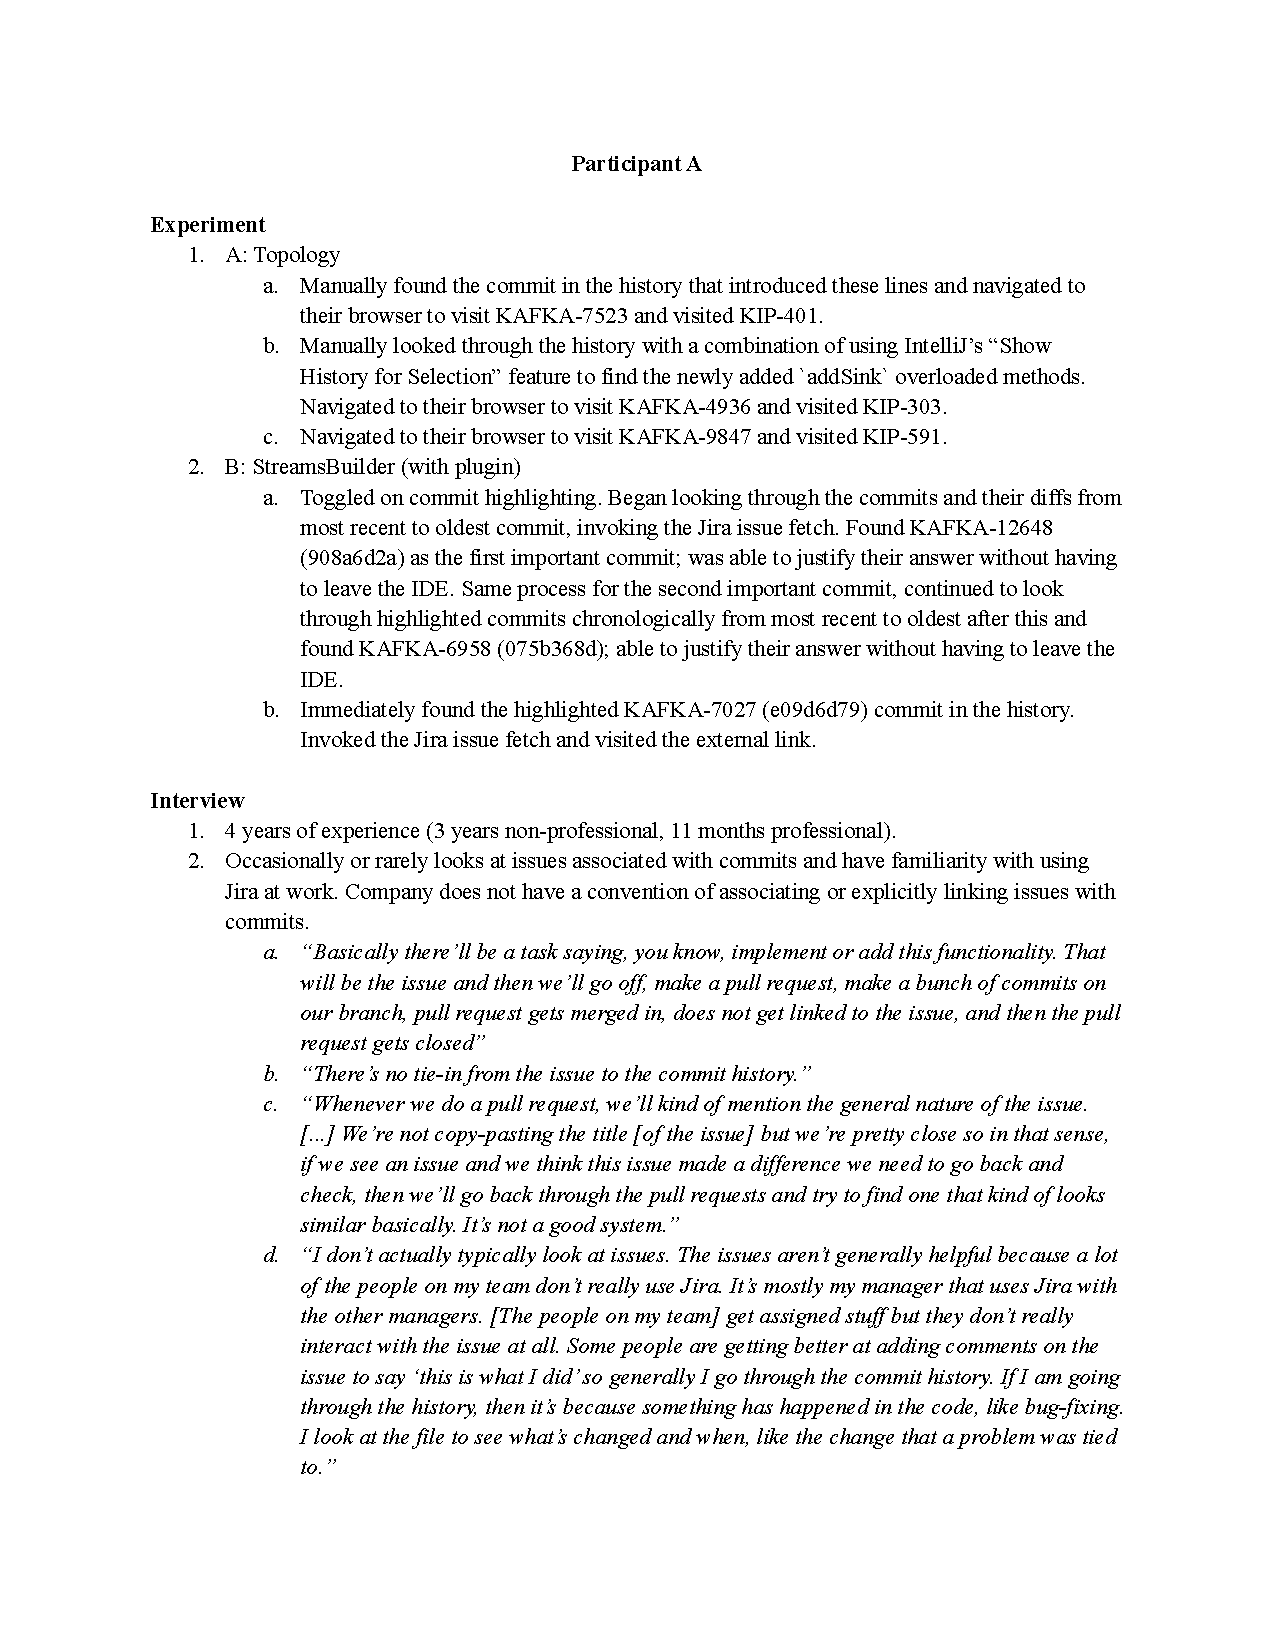
\includegraphics[page=1,width=\textwidth]{./files/session-summaries.pdf}
\end{figure}

\begin{figure}[H]
    \includegraphics[page=2,width=\textwidth]{./files/session-summaries.pdf}
\end{figure}

\begin{figure}[H]
    \includegraphics[page=3,width=\textwidth]{./files/session-summaries.pdf}
\end{figure}

\begin{figure}[H]
    \includegraphics[page=4,width=\textwidth]{./files/session-summaries.pdf}
\end{figure}

\begin{figure}[H]
    \includegraphics[page=5,width=\textwidth]{./files/session-summaries.pdf}
\end{figure}

\begin{figure}[H]
    \includegraphics[page=6,width=\textwidth]{./files/session-summaries.pdf}
\end{figure}

\begin{figure}[H]
    \includegraphics[page=7,width=\textwidth]{./files/session-summaries.pdf}
\end{figure}

\begin{figure}[H]
    \includegraphics[page=8,width=\textwidth]{./files/session-summaries.pdf}
\end{figure}

\begin{figure}[H]
    \includegraphics[page=9,width=\textwidth]{./files/session-summaries.pdf}
\end{figure}

\begin{figure}[H]
    \includegraphics[page=10,width=\textwidth]{./files/session-summaries.pdf}
\end{figure}

\begin{figure}[H]
    \includegraphics[page=11,width=\textwidth]{./files/session-summaries.pdf}
\end{figure}

\begin{figure}[H]
    \includegraphics[page=12,width=\textwidth]{./files/session-summaries.pdf}
\end{figure}

\begin{figure}[H]
    \includegraphics[page=13,width=\textwidth]{./files/session-summaries.pdf}
\end{figure}

\begin{figure}[H]
    \includegraphics[page=14,width=\textwidth]{./files/session-summaries.pdf}
\end{figure}

\begin{figure}[H]
    \includegraphics[page=15,width=\textwidth]{./files/session-summaries.pdf}
\end{figure}

\begin{figure}[H]
    \includegraphics[page=16,width=\textwidth]{./files/session-summaries.pdf}
\end{figure}

\begin{figure}[H]
    \includegraphics[page=17,width=\textwidth]{./files/session-summaries.pdf}
\end{figure}

\begin{figure}[H]
    \includegraphics[page=18,width=\textwidth]{./files/session-summaries.pdf}
\end{figure}

\begin{figure}[H]
    \includegraphics[page=19,width=\textwidth]{./files/session-summaries.pdf}
\end{figure}

\begin{figure}[H]
    \includegraphics[page=20,width=\textwidth]{./files/session-summaries.pdf}
\end{figure}

%%%%%%%%%%%%%%%%%%%%%%%%%%%%%%%%%%%%%%%%%%%%%%%%%%%%%%%%%%%%%%%%%%%%%%
\endinput